\chapter{Le Magnétisme Moléculaire}

Pour mériter le nom d'aimant moléculaire, une molécule doit remplir plusieurs critères. Bien s\^ur, il faut qu'elle possède un moment magnétique non nul qui peut \^etre de spin et/ou orbital. Il faut de plus, que ce moment magnétique est une orientation préférentielle. Cela se traduit par l'existence d'un axe facile, c'est à dire deux orientations qui correspondent à un minimum d'énergie. En outre, l'anisotropie, c'est à dire la barrière d'énergie séparant les deux orientations, doit \^etre suffisamment grande pour que l'énergie thermique ne puisse pas retourner l'aimantation.

On souhaite aussi pouvoir mettre en évidence des phénomènes quantiques tel que le retournement de l'aimantation par effet tunnel~(ou Quantum Tunneling of the Magnetization - QTM) ou bien encore la phase de Berry. Ceci n'est possible que s'il existe un couplage entre les différents états du système. Celui-ci a généralement pour origine la presence d'un plan difficile qui va introduire des termes création/annihilation dans la description du système.

Le spin électronique n'est pas toujours l'unique acteur du magnétisme moléculaire. Il arrive que le spin nucléaire, au travers du couplage hyperfin, joue un r\^ole majeur dans les phénomènes quantique et les propriétés magnétiques mesurés.

Afin de comprendre la physique associé aux aimants moléculaires, on peut donc procéder par étape. On peut tout d'abord décrire l'origine physique du moment magnétique d'une molécule. On peut ensuite introduire la notion d'axe facile et voir comment cette notion se traduit dans le formalisme quantique. On peut ensuite aborder la notions de plan difficile, son origine et ces conséquences. Enfin, une description des interaction entre spin électronique et spin nucléaire est nécessaire pour décrire de la façon la plus complète certains aimants moléculaire, à base de lanthanide notamment.

\section{L'origine du moment magnétique}
Pour obtenir un aimant moléculaire, deux stratégies peuvent être adoptés. La première consiste à synthétiser une molécule composé de plusieurs atomes magnétique qui vont interagir entre eux, par l'intermédiaire des ligands, pour donner un moment magnétique résultant non nul. La deuxième technique consiste à n'utiliser qu'un atome métallique magnétique que l'on va venir entourer de ligands non magnétiques.

\subsection{La solution a plusieurs centres}
Cette solution a été la première adopté dans le domaine du magnétisme moléculaire. Elle a permis notamment de synthétiser la désormais célèbre molécule de Mn$_{12}$-ac~(cf Fig.\ref{Mn12}). Cette dernière est composé de douze atomes de Manganèse et autant d'atomes d'oxygène~(qui consituent le coeur magnétique) ainsi que des ligands organiques. Les huit atomes de manganèse en périphérie, de part leur interaction, sont parallèles les uns au autres. Chacun d'eux possédant un spin $S=2$, on se retrouve avec un spin total $S=16$. Les trois atomes situés au centre du coeur magnétique sont également alignés entre eux pour un spin total de $S=6$~(pour chaque manganèse $S=3/2$). Ces deux groupes étant antiparallèle l'un par raport à l'autre, on obtient un spin total de $S=10$. Dans cet exemple, les atomes d'oxygène jouent un r\^ole majeur au travers de l'interaction dite de "super échange" qui lie les différents atomes de manganèses entre eux.
\begin{figure}
\centering \includegraphics[scale=0.3]{Theorie/MagMol/figure1/Mn12.png} 
\caption{Sur la gauche, la molécule de Mn$_{12}$-ac. Sur la droite, le centre magnétique Mn$_{12}$O$_{12}$. Les quatre manganèses internes de spin $S=3/2$ sont antiparallèles aux huit maganèses de spin $S=2$ situés en périphérie. Le moment magnétique total résultant est $S=10$~(extrait de When Magnetism Goes Nano). Le couplage entre les différents spins est médié par les atomes d'oxygène en bleus sur la figure.}
\label{Mn12}
\end{figure}

\subsection{La solution de l'ion métallique unique}
Dans ce deuxième type d'aimants moléculaires, le moment magnétique total ne dépend que de celui de l'ion qui la compose. Cet ion va \^etre ensuite inséré dans un ligand pour former un aimant moléculaire. Contrairement à ce qui a été présenté précédemment, le moment magnétique total ne dépend donc pas des interactions entre différents centre magnétique. On peut dors et déjà y voir un signe de robustesse, ce type d'aimant moléculaire étant par construction, moins sensible à une déformation de sa structure~(cf chapitre précédent avec l'effet Jhan-Teller). Parmis les molécules les plus étudiées , on trouve le "double-decker"~(nommé en référence aux avions à deux ailes) où plusieurs ion peuvent \^etre choisi comme centre magnétique. Dans notre cas, nous utiliserons le TbPc$_2$ où terbium "double-decker".



\section{Hamiltonien d'un aimant moléculaire "standard"}
\subsection{L'axe facile}
Le champ de ligand a une influence majeure sur le magnétisme de la molécule. Celle-ci peut \^etre prise en compte par l'introduction des opérateurs de Stevens~(rappelé en annexe) qui tiennent compte des symétries du système. Pour notre introduction, nous allons nous concentrer sur un terme simple introduisant un axe facile à savoir:
 \begin{eqnarray}
E_{ani} = -DS_z^2 \nonumber
\end{eqnarray}
où $D$ est le paramètre d'anisotropie, $S_z$ la composante en $z$ du moment magnétique et $E_{ani}$ la modification de l'énergie du système du à cette anisotropie. Si $D<0$, nous avons à faire à un axe difficile et le moment magnétique se trouvera de préférence dans le plan perpendiculaire à l'axe $z$. Si $D>0$, nous avons un axe facile et le moment magnétique sera aligné le long de l'axe z.

La Fig.\ref{Fe8Zeeman}.a présente la position en énergie des différents états $|m_z \langle$ dans le cas $S=10$ et $D>0$. On remarque que les deux orientations préférentielles $m_z=10$~(up) et $m_z=-10$~(down) sont séparés par une barrière d'anisotropie de hauteur $|D|S^2$.

\begin{figure}
\centering 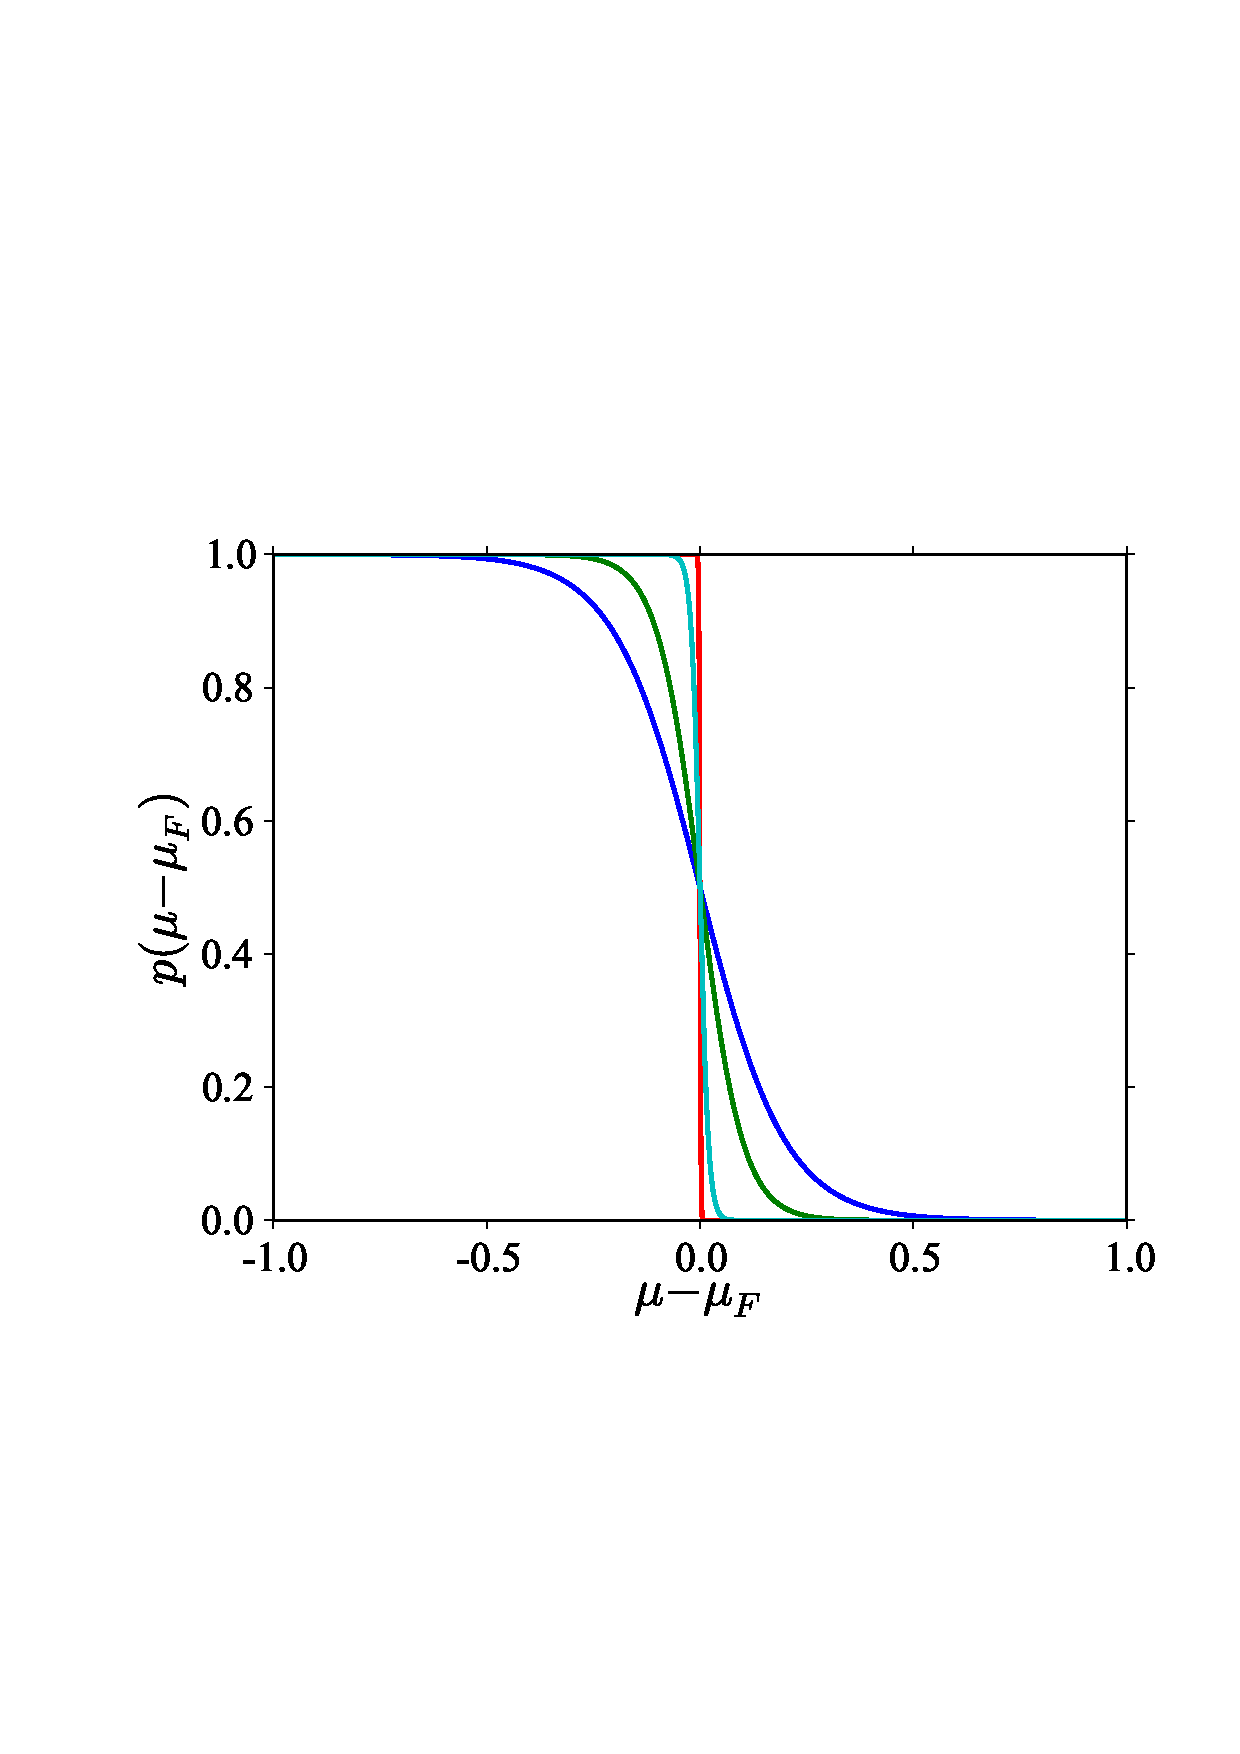
\includegraphics[scale=0.3]{Theorie/MagMol/figure2/figure2.png} 
\caption{A gauche, structure générale d'un "double decker" à base de Lanthanide~(noté Ln - tiré de Ishikawa, Single molecule magnet with single lanthanide ion). A droite, vu d'artiste de cette m\^eme molécule. Les atomes d'azote sont représentés en bleu, ceux de carbone en noir, ceux hydrogènes en beige et l'atome lanthanide en mauve}
\label{TbPc2}
\end{figure}

\subsection{Le plan difficile}
De m\^eme que nous pouvons avoir un axe facile( ou difficile), on peut égalment rencontrer un plan difficile(~ou facile). Il peut \^etre exprimé deux façons rigoureusement équivalente :
\begin{eqnarray}
E_{\perp} = E ( S_x^2 -S_y^2)  = \frac{E}{2} ( S_+^2  + S_-^2) \nonumber 
\end{eqnarray}
où $S_x$ et $S_y$ sont les projection du moment magnétique dans le plan $(x,y)$, $S_+$ et $S_-$ les opérateurs création anhilation, $E$ est le paramètre d'anysotropie et $E_{\perp}$ l'énergie associé à la présence d'un plan difficile. La présence des termes création anhilation n'est pas sans conséquence sur le système. En effet, ces termes vont venir coupler les différentes valeur $m_z$.

\subsection{L'effet Zeeman}
Comme tout système magnétique, un aimant moléculaire est sensible à l'effet Zeeman. Celui si va venir faire varier l'énergie du système de la valeur
\begin{eqnarray}
E_{z}= g\mu_b \mathbf{BS} \nonumber
\end{eqnarray}
ou $E_{z}$ est l'énergie associé à l'effet Zeeman, $g$ le facteur de Landé, $\mu_b$ le magnéton de Bohr, $B$ le champ magnétique appliqué et $S$ le moment magnétique du système. Si maintenant ce champ magnétique est appliqué celon l'axe $z$ du système, cette expression devient :
\begin{eqnarray}
E_{z}= g\mu_b B S_z \nonumber
\end{eqnarray}

\subsection{La cas du Fe$_8$}
Si l'on synthétise ce qui vient d'\^etre présenté, un aimant moléculaire soumit à un champ magnétique $B$ appliqué suivant l'axe $z$ possède l'hamiltonien suivant:
\begin{eqnarray}
E =  -DS_z^2 + \frac{E}{2} ( S_+^2  + S_-^2) + g\mu_b B S_z 
\end{eqnarray}


Nous allons maintenant appliqué cet hamiltonien à l'étude d'un aimant très utiliser dans les expériences relativer au magnétisme moléculaire : le Fe$_8$. Nous avons déjà vu l'influence de l'effet Zeeman et de l'axe facile sur les spectre en énergie d'un système. Ici, nous allons nous intéresser plus particulièrement à la présence d'un plan difficile est voir comment se plan vient perturber le système. La présence de ces anti-croisements témoigne du couplage entre les différents état de l'aimantation du système. Nous allons à present étudier les conséquence d'un tel couplage.

\begin{figure}
\centering \includegraphics[scale=0.5]{Theorie/MagMol/figure3/figure3.pdf} 
\caption{Sur la gauche, la molécule de Mn$_{12}$-ac. Sur la droite, le centre magnétique Mn$_{12}$O$_{12}$. Les quatre manganèses internes de spin $S=3/2$ sont antiparallèles aux huit maganèses de spin $S=2$ situés en périphérie. Le moment magnétique total résultant est $S=10$~(extrait de When Magnetism Goes Nano). Le couplage entre les différents spins est médié par les atomes d'oxygène en bleus sur la figure.}
\label{Fe8Zeeman}
\end{figure}

\subsection{les anti-croisement}
Au niveau d'un anti-croisement, les états propres du système ne sont plus les états magnétique ($S,S_z$) mais plutot une combinaison de ces états. Si l'on se place loin de l'anti-croisement, les états $m$ et $m'$ sont les états propre du système. Mais plus on se rapproche de l'anti-croisement plus les états sont mélange pour anteindre un maximum d'intrication quand la séparation en énergie entre les deux niveau est minimale.

Lorsque l'on balaie le champ magnétique autour d'un tel anti-croisement, il y a une certaine probabilité de passer de l'état $m$ à l'état $m'$ et vice-versas. Cette probabilité est régie par la formule de Landau-Zenner qui dépend à la fois de la séparation minimale entre les deux niveaux ainsi que de la vitesse de balayage du champ magnétique. Cette probabilité peut s'exprimer de la façon suivante :
\begin{eqnarray}
P = 1 - \exp \left( -\frac{\pi \Delta^2_{mm'}}{2 \hbar g \mu_B |m-m'|\frac{dH_z}{dt}} \right)
\end{eqnarray}
ou P est la probabilité de passer de l'état $m$ à l'état $m'$, $\Delta_{mm'}$ l'écart minimum en éngergie entre les deux niveaux, $\frac{dH_z}{dt}$ la vitesse de balayage en champ magnétique. On constate tout d'abord que si la vitesse est très faible, la probabilité de passer d'un état à l'autre est de 1. On retrouve ici le théorème adiabatique. A l'autre bout de l'échelle, si je balaie très rapidement le champ magnétique cette probabilité devient nulle. Tout se passe comme si l'on avait été si vite que le système n'avait pas eu le temps de "sentir" l'anti-croisement.

\subsection{Mesure de l'aimantation}

A FAIRE!!!!!!

\section{Le Terbium double-decker ou TbPc$_2$}

\subsection{Origine du moment magnétique}
Le terbium double-decker est un aimant moléculaire dont le moment magnétique est d\^u à un centre magnétique unique : l'ion Tb$^{3+}$. L'atome de Terbium possède un noyau relativement lourd et le couplage spin orbite joue donc un r\^ole prépondérant dans les propriété magnétique de ce dernier. Le moment magnétique fondamental total de cet ion peut \^etre déterminer par un calcul relativement complexe. La théorie donnent un moment total $J=6$ pour l'état fondamental ainsi qu'une séparation en énergie de plusieurs millier de Kelvin entre celui-ci et le premier état excité $J=5$. On peut donc sans trop de risque négliger les états excité et considéré uniquement la configuration $J=6$. Ce moment provient du moment angulaire électronique~($L=3$) ainsi que des six spins électroniques non appariés. 

\begin{figure}
\centering \includegraphics[scale=0.5]{Theorie/MagMol/figure4/figure4.pdf} 
\caption{Sur la gauche, la molécule de Mn$_{12}$-ac. Sur la droite, le centre magnétique Mn$_{12}$O$_{12}$. Les quatre manganèses internes de spin $S=3/2$ sont antiparallèles aux huit maganèses de spin $S=2$ situés en périphérie. Le moment magnétique total résultant est $S=10$~(extrait de When Magnetism Goes Nano). Le couplage entre les différents spins est médié par les atomes d'oxygène en bleus sur la figure.}
\label{TbPc2Zeeman}
\end{figure}

\subsection{Hamiltonien}

\subsubsection{Le moment magnétique électronique}
L'Hamiltonien relatif au TbPc$_2$ est plus complexe que ce qui a été présenté précédemment. Il est pour cela plus pratique de faire appel aux opérateur de Stevens afin d'obtenir une écriture plus concise.

L'Hamiltonien relatif à la présence d'un axe facile s'exprime comme suit :
\begin{eqnarray}
H_{//} = \alpha A_2^0 \langle r^2 \rangle O_2^0 + \beta A_4^0 \langle r^2 \rangle O_4^0 + \gamma A_6^0 \langle r^2 \rangle O_6^0
\end{eqnarray}
ou les différent $O_i^0$ sont les opérateurs de Stevens, $A_i^0$ les coéfficient relatifs à la molécule de TbPc$_2$ et $\alpha$, $\beta$ et $\gamma$ les coéfficient introduit par Stevens. Les opérateur $O^0_i$ sont basé sur des sommes d'opérateur $S_z^{2n}$. Il s'agit donc d'un opérateur diagonal qui ne vient pas coupler les différents état de la base ($J$,$J_z$) entre entre eux. Le diagramme Zeeman correspondant est donné dans la Fig.\ref{TbPc2Zeeman}.a.

Les états fondamentaux $J_z = \pm 6$ sont isolé des états excités par une énergie de plus de $600$\,K. Puisque nos expérience se font dans le domaine du sub-Kelvin, on peut négliger les états excité et nous concentrer sur les deux états fondamentaux  $J_z = \pm 6$.

La présence d'un plan difficile, nécessite l'introduction d'un terme suplémentaire :
\begin{eqnarray}
H_{\perp} = \beta A_4^4 \langle r^2 \rangle O_4^4
\end{eqnarray}
où la m\^eme notation a été utilisé. Ce dernier terme ne modifie pas l'allure générale du diagramme Zeeman. En revanche, il introduit un couplage entre les états  $J_z = \pm 6$ qui se traduit par la présence d'anti-croisement comme le montre la figure\ref{TbPc2Zeeman}.b.

\subsubsection{Le spin nucléaire}
Les orbitale électronique étant de type 4f, leur interaction avec le spin nucléaire doit \^etre prise en compte. Dans le cas du terbium, le spin nucléaire est de $I = 3/2$. Du fait de ça forme allongé, il possède élgalement un moment quadripolaire de sorte que l'hamiltonien relatif au spin nucléaire est donné par :
\begin{eqnarray}
H_I = P\left(I_z^2 - \frac{1}{3}I(I+1)\right)
\end{eqnarray}
où $P$ est le moment quadripolaire et un terme constant a été ajouté pour garder le barycentre des énergie à zéro.

De plus, ce spin nucléaire interagit avec le moment magnétique électronique au traver de l'interaction hyperfine. Un terme rendant compte de cette interaction doit donc \^etre introduit. Son expression est simple et ne met en jeux que le produit scalaire des deux spin :
\begin{eqnarray}
H_{hf} = A_{hf}\mathbf{J}\mathbf{I}
\end{eqnarray}
où $\mathbf{J}$ et $\mathbf{I}$ sont respectivement le moment magnétique électronique et le spin nucléaire, $A_{hf}$ étant la constante d'interaction hyperfine.

\subsubsection{L'Hamiltonien de l'aimant moléculaire}

Ces différents terme doivent bien s\^ur \^etre inclus dans l'Hamiltonien total de l'aimant moléculaire. Cela donne, en reprenant la notion précédente
\begin{eqnarray}
H = H_z + H_{//} + H_{\perp} + H_{hf}
\end{eqnarray}
Les trois derniers terme n'agissent que comme une perturbation et l'allure générale présenté dans la figure??.a n'est pas altéré. On peut donc continuer à ce concentrer sur les seuls états $J_z = \pm 6$. A cette échelle en revanche, les effets ne sont plus négligeable. En plus de l'anti-croisement introduit par la présence du plan difficile, le couplage hyperfin vient diviser les états fondamentaux  $J_z = \pm 6$ en deux jeux de quatre états, chacune de ces quatre états étant relatif à un état de spin nucléaire. De plus, pour un m\^eme état de spin nucléaire, l'anti-croisement entre les états de  $J_z = \pm 6$ sont conservé. En revanche, seul des croisements sont observés pour les état de spin nucléaire différents~(cd Fig. \ref{TbPc2Zeeman}.c).

\subsection{Mesure de l'aimantation}

A FAIRE!!!